\documentclass[12pt]{article}
\usepackage{import}
\usepackage{preamble}

\begin{document}

\import{./}{title.tex}

\pagenumbering{roman}

%----------------------------------------------------------------------------------------
%	ACKNOWLEDGEMENTS
%----------------------------------------------------------------------------------------
\section*{Acknowledgements}
I would like to thank Dr Peter Blanchfield, Prof. Paul McGraw and Dr Denis Schluppeck, School of Psychology, providing the data and the opportunity to undertake this project.
\\
\\
I would also like to thank everyone at the University of Nottingham school of computer science as well as the computer science master class 2018 for making my time here a truly memorable experience. In particular, I express my deep gratitude to Dr Gail Hopkins, Dr Mercedes Torres Torres, Dr Jérémie Clos and Professor Alexander Foss from department of ophthalmology for their guidance and advice throughout the project.
\addcontentsline{toc}{section}{Acknowledgements}



%----------------------------------------------------------------------------------------
%	DECLARATION PAGE
%----------------------------------------------------------------------------------------
\begin{textblock*}{\textwidth}(24mm,148mm)
\section*{Declaration}
I declare that this thesis has been composed solely by myself and that it has not been submitted, in whole or in part, in any previous application for a degree. Except where states otherwise by reference or acknowledgment, the work presented is entirely my own.
\end{textblock*}
\addcontentsline{toc}{section}{Declaration}





\newpage
%----------------------------------------------------------------------------------------
%	ABSTRACT PAGE
%----------------------------------------------------------------------------------------
\section*{Abstract}
Strabismus can cause blind. 
\addcontentsline{toc}{section}{Abstract}
\newpage

%----------------------------------------------------------------------------------------
%	Abbreviations
%----------------------------------------------------------------------------------------

\section*{}
\nomenclature[z-SVM]{SVM}{Support vector machine}
\nomenclature[z-SVR]{SVR}{Support vector regression}
\nomenclature[z-PCA]{PCA}{Principal competent analysis}

\printnomenclature
\addcontentsline{toc}{section}{Abbreviations}


\newpage


%----------------------------------------------------------------------------------------
%	LIST OF CONTENTS/FIGURES/TABLES PAGES
%----------------------------------------------------------------------------------------
\pagenumbering{gobble}
\tableofcontents
\listoffigures
\listoftables

\newpage



\pagenumbering{arabic}
\section{Introduction}
Strabismus, commonly known as squint or crossed eye, are estimated to affect 2.5\% of the children in developed western countries \citep{Williams2008a,Torp-Pedersen2017}. Strabismus may cause individual develop amblyopia. An accurate and early diagnosis of strabismus is important to prevent individual to develop amblyopia which could lead irreversible vision loss later in life. It is also important in preventing development into number of medical complication and psychosocial impact cause by strabismus. 

A number of clinical methods, orthoptic assessment, are currently use by orthoptist to assessed strabismus and to determine the angle of ocular deviation. In contrast to manual diagnosis, automatic recognition can significantly reduce labour cost and increase diagnosis efficiency. \citet{Bakker2013, Chen2018} has have devised such methods with using three camera to identify and measure angles of strabismus fast and accurately. Furthermore it being able to operate independently from the head pose.
%\citet{Chen2018} has devised such method to recognise strabismus using eye-tracking data and convolutional neural networks 

%As the costs of technology decline, an increasing amount of data become available. Additionally, as machine learning algorithm become more mature and their ability to predict results almost as good as, and in some cases better than, humans in certain specific tasks. (need some supporting evidences)

However, individuals having the same type of strabismus with same degree of ocular deviation had been observed with significantly different depth and distance perception (evidence other than \citep{Hussain2018}). One could be suppression. Another a known complication cause by strabismus known as abnormal retinal correspondence. Therefore 
Therefore, a computerised visual test \citep{Hussain2018} to that estimate one's distance perception combining with fMRI scan. By gaining greater understanding of how one visual cortex has been alter would allow a better target treatment.
talking about test we want to do\\
-significance of data collected
aim and objective (basically repeat the project plan).
objective1- literature of the medical discuss in section 2
valid thier data set
objective2- statistical 
objective

aesthetic to fix

\newpage
\section{Background}
    \subsection{Strabismus}
        As previously mention strabismus, commonly known as squint or crossed eye, is a condition in which the eyes don’t line up to work in synchronous fashion. It is not to be confused with amblyopia, also known as lazy eye, is a vision development disorder in which an eye fails to achieve normal visual acuity, even with prescription eyeglasses or contact lenses.\\
        
        There are numerous reasons could give rise of strabismus. They include genetics, inappropriate development of the "fusion center" of the brain, problems with the controlled center of the brain, injuries to muscles or nerves or other problems involving the muscles or nerves.
        The ocular posture is controlled by the six extraocular muscles, the four recti and two obliques. Pulleys of connective tissue attached to orbital bones and extraocular muscles form a fascial sling around the globe which helps to maintain ocular position figure \ref{fig:eye_muscles}.
        \begin{figure}[h]
            \centering
            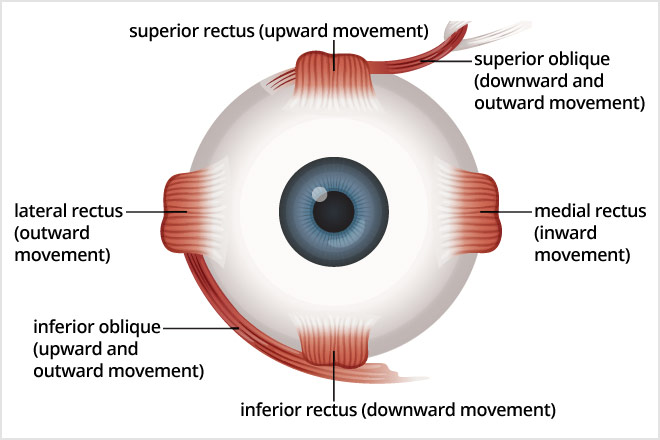
\includegraphics[width = 0.8\textwidth]{Images/eye_muscles.png}
            \caption{Anterior view of the right eye}
            \label{fig:eye_muscles}
            \raggedright \footnotesize Showing the orientation of the extra-ocular muscles and their indicate directions of eye movement produced by contractions of the individual muscles.
        \end{figure}
        \\
        Strabismus is classified by the direction of the deviation: when one eye looks directly at the object you are viewing, while the other eye is misaligned inward (esotropia, "crossed eyes" or "cross-eyed"), outward (exotropia or "wall-eyed"), upward (hypertropia) or downward (hypotropia) figure \ref{figure:strabismus_type}.
        Diagnosis 
        The angle of deviation can range from 2 to 20 prism dioptres. The most frequently used method, despite having some deficiency, is the alternate prism cover test (APCT). It is also used to measure the angle of deviation in patients with strabismus.
        occurs when light that enters the eye is improperly
\begin{figure}[h!]
\centering
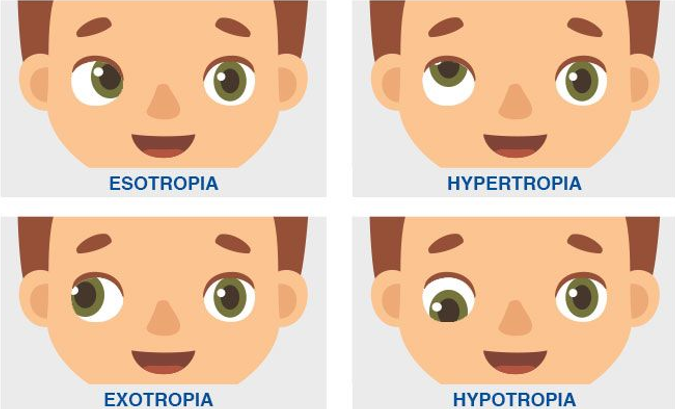
\includegraphics[width =0.9\textwidth]{Images/stranismus.png}
\caption{Type of Strabismus} \label{figure:strabismus_type}
\raggedright
\footnotesize
clockwise

\end{figure}
    \subsubsection{Image formation principle}

    \subsubsection{Introduction to visual pathway}
    

Under normal circumstances, the brain develops to correlate the visual input at each fovea coming from straight in front. 

The left visual field stimulates nasal retina in the left eye and temporal retina in the right eye. Connected and perceived by the right hemisphere of our brain's visual cortex 
The right visual field stimulate the temporal retina in the left eye and nasal retina in the right eye. 

    \begin{figure}[h!]
        \centering
        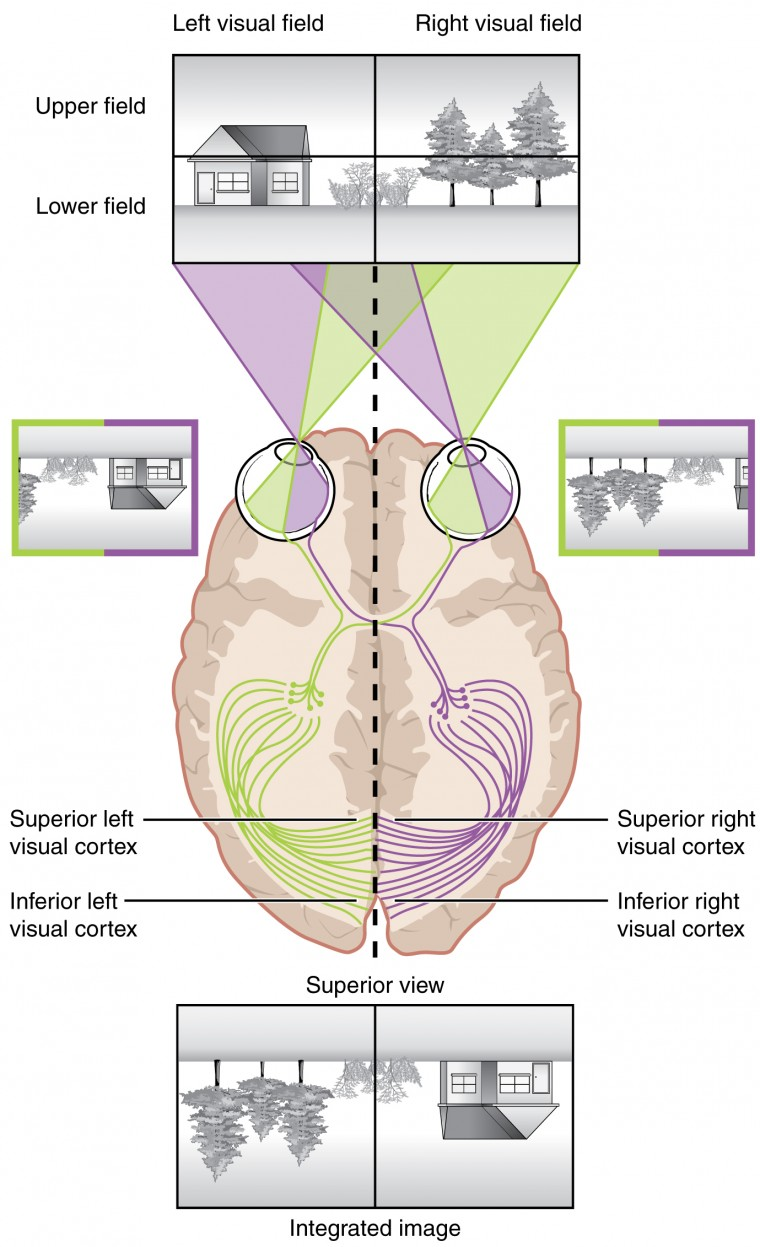
\includegraphics[width=0.7\textwidth]{Images/Topographical_Image_on_Retina.jpg}
        \caption{Caption}
        \label{fig:retina_topographic}
    \end{figure}
\subsection{Statistical analysis/data pre-processing}
- how data collected
- what we need to do - remove outlier
- measure angle and distance from centriaity

\subsection{Machine learning}
\subsubsection{Subsection}
\paragraph{Subsubsection}
\newpage

\section{Specification, Design, Implementation.}
specification == objective
design = mathematical background , for function how functions work (what kind of built in function used and what do they do(what purpose do they serve))
\subsection{Statistical analysis/data pre-processing}
- what it is look like

\newpage

\section{Evaluation}
Has the aim been achieved? You should be able to provide an objective evaluation of whether the project was a success. (Could be experimental evaluation, or a proof, or a user study.)

\section{Conclusions}

\newpage
\bibliographystyle{agsm}
\bibliography{references,mendeley}

\appendix
\section*{Appendices}
\addcontentsline{toc}{section}{Appendices}
\renewcommand{\thesubsection}{\Alph{subsection}}
\appsection{Code}

\end{document}